\documentclass[a4paper]{article}

  \usepackage{fullpage} % Package to use full page
  \usepackage{parskip} % Package to tweak paragraph skipping
  \usepackage{tikz} % Package for drawing
  \usepackage{amsmath}
  \usepackage{siunitx}
  \usepackage{amsfonts}
  \usepackage{amssymb}
  \usepackage{hyperref}
  \usepackage[utf8]{inputenc}
  \usepackage[english]{babel}
  \usepackage{multicol}
  \usepackage{graphicx}
  \graphicspath{ {./images/} }
  
  \newcommand\tab[1][0.5cm]{\hspace*{#1}}
  
  \title{Laboratory 8: Transient Responses of First Order RL and RC Circuits}
  \author{Adrian Darian}
  \date{12/2/2020}
  
  \begin{document}
  
\maketitle
  
\section*{Objectives}
• Observe the transient responses of RL and RC circuits. \\
• Learn to how to measure time constant of first order circuits. \\

\section*{Equipment and components}
• A computer \\
• PSPICE software \\

\section*{Preliminary}
• Read the lecture slides of "Inverse Laplace Transform and RC, RL, and RLC Circuits".\\
• Calculate the time constant when $R = 1 \si{\kilo\ohm}, C = 0.5 \si{\mu}F, C = 1 \si{\mu}F, and C = 2 \si{\mu}F$, respectively. Fill in Table 1. Refer to the natural and step responses of RC circuits shown below for finding the time constant. \\
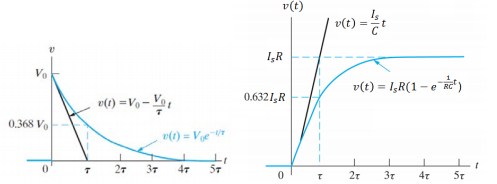
\includegraphics[scale=0.5]{image-1.png} \\
• Calculate the time constant when $R = 10 \si{\ohm}, L = 10 mH, L = 20 mH, and L = 40 mH$, respectively. Fill in Table 2. Refer to the above two graphs to find the time constant for RL circuits. \\
• Pulse waveform: A voltage pulse source can be applied using VPULSE element in PSpice. VPULSE has 7 parameters that are described and shown below. \\
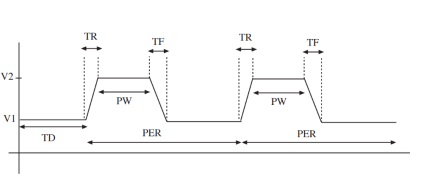
\includegraphics[scale=0.5]{image-2.png} \\
As an example, a square waveform can be created by setting $TR = TF = 0$ and $PER = 2 PW$. $TD$ is the delay time \\

\section*{Procedure}
\begin{itemize}
	\item[1.] Open PSpice and construct a circuit shown below with a resistor of $1 \si{\kilo\ohm}$ and a capacitor of $1 \si{\mu}F$. $V_{g}$ is an independent voltage source generating square waveforms. Set $TR = TF = TD = 0, V_{1} = 0, and V_{2} = 10 V$ Wisely set the period of the waveform so that you can clearly observe the natural and step responses $v(t)$ of the RC Circuit. \\
	      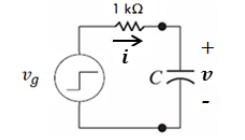
\includegraphics[scale=0.5]{image-3.png} \\   
	\item[2.] Measure $i(t)$ and $v(t)$. Plot them. What did you find? Why? \\
	\item[3.] Fill the simulation results in Table 1 \\
	      \begin{tabular}{|c|c|c|c|}
	      	\hline
	      	Resistance ($\si{\kilo\ohm}$) & Capacitance ($\si{\mu}F$) & Calculated Time Constant ($ms$) & Measured Time Constant ($ms$) \\
	      	\hline
	      	1                             & 0.5                       & 0.5                             & 1                             \\
	      	\hline
	      	1                             & 1                         & 1                               & 0.5                           \\
	      	\hline
	      	1                             & 2                         & 2                               & 2                             \\
	      	\hline
	      \end{tabular} \\
	\item[4.] let $R = 1 \si{\kilo\ohm} and TR = TF = TD = 0, V_{1} = 0, V_{2} = 10 V, and PER = 2 ms$, select the capacitance of the capacitor so that the response $v(t)$ of the circuit is a triangle waveform, as shown below. \\
	      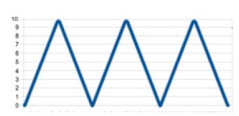
\includegraphics[scale=0.5]{image-4.png} \\  
	\item[5.] Construct a circuit shown below with a resistor of $10 \si{\kilo\ohm}$ and an inductor of $10 mH$. Set $TR = TF = TD = 0, V_{1} = 0, V_{2} = 10 V$ for the pulse voltage source. Wisely select it pulse width so that you can clearly observed the responses of the RL circuit. \\
	      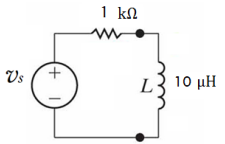
\includegraphics[scale=0.5]{image-5.png} \\ 
	\item[6.] Measure the current $i(t)$ in the circuit and voltage $v(t)$ across the inductor. Then plot them. What did you find? Why? \\
	\item[7.] Fill the simulation results in Table 2 \\ 
	      \begin{tabular}{|c|c|c|c|}
	      	\hline
	      	Resistance ($\si{\ohm}$) & Capacitance ($mH$) & Calculated Time Constant ($ms$) & Measured Time Constant ($ms$) \\
	      	\hline
	      	10                       & 10                 & 100                             & 200                           \\
	      	\hline
	      	10                       & 20                 & 200                             & 100                           \\
	      	\hline
	      	10                       & 30                 & 300                             & 300                           \\
	      	\hline
	      \end{tabular} \\
\end{itemize}

\section*{Questions and Conclusions}
• Summarize your findings and explanations in response to the questions posed in this lab.  \\
In this lab I learned more about how a capacitor works in a practical stand point. I really found out that capacitors work different from one another and the data fluxtuates frequently. This is primarily due to the sinusoidal power source. Whenever I flipped the switch back and forth the readings would scatter and then slowly realign. In the end the larger the capcitor the longer a light can be charged.
\end{document}